\subsection{Программная реализация устройства стратегического управления}
Устройством стратегического управления является одноплатный миникомпьютер «Rasp- berry Pi Zero W 2» (Рисунок 3.3), система запускается сразу после подачи питания на устройство. Происходит запуск операционной системы «Linux» и ожидание подключения пользователя к устройству. Возможен два варианта использования стратегического устройства:

\begin{enumerate}
	\item Подключение по беспроводному каналу, по протоколу SSH.
	\item Через проводное подключение, путем подключения проводов монитора и устройств ввода/вывода.
\end{enumerate}

Для подключения мини-компьютера по беспроводному каналу, необходимо чтобы микрокомпьютер был в локальном окружении беспроводной сети.

Для дальнейшей работы управления используется один из языков высокого уровня, например, язык программирования Python c использованием библиотек, пример представлен на рисунке \ref{CodePython1}.
\begin{figure}[H]
	\centering

	\begin{minted}[tabsize=2,breaklines,fontsize=\small]{python}
import numpy as np
from pybotics.geometry import vector_2_matrix
poses = np.array([
    vector_2_matrix([600, -150, 800,
                     np.deg2rad(-90), 0,
                     np.deg2rad(-90)]),
    vector_2_matrix([700, -150, 800,
                     np.deg2rad(-90), 0,
                     np.deg2rad(-90)])
])
start_end_joints = [robot.ik(p) for p in poses]
	\end{minted}
	\caption{Фрагмент использования сторонних библиотек на языке питон.}\label{CodePython1}
\end{figure}


При помощи библиотек возможно производить программирование робота в режиме симуляции и только потом генерировать команды для контроллера тактического управления. Использования языка высокого уровня позволяет создавать комплексные стратегии движения и обрабатывать сложные алгоритмы. Для коммуникации между устройствами стратегического и тактического уровня предполагается использование написанного библиотеки API, пример функции представлен на Рис. \ref{CodePython2} для общения между микроконтроллером и микрокомпьютера


\begin{figure}[H]
	\centering

	\begin{minted}[tabsize=2,breaklines,fontsize=\small]{python}
def send_movej_command(self, command):
    """
    Send a moveJ command to the robot through the serial connection.
    Args:       
    serial_connection (serial.Serial): The serial connection to the robot.
    command (str): The moveJ command string.
    """
    with serial.Serial(self.serial_port, self.baud_rate, timeout=1) as ser:
  	log("Serial connection established.")
    serial_connection.write(command.encode())
    	log(f"Sent command: {command}")
    if self.ser.in_waiting:
	response = self.ser.read(ser.in_waiting).decode()
          log("Received response:", response)
	\end{minted}
	\caption{Фрагмент функции API библиотеки для использования на языке Python.}\label{CodePython2}
\end{figure}


Так же ещё одним возможным видом программирования является использование программного обеспечение RoboDK, на устройстве стратегического управления исполняется драйвер, который передает данные из сокетного TCP/IP соединения в Uart, список команд рассматривается в таблице 5.1 на контроллер тактического управления фрагмент представлен в приложение 2.

\begin{table}[H]
	\caption{Список базовых команд который поддерживает robotDK}\label{TRobotDK}
	\begin{adjustbox}{width=\textwidth}

		\begin{tabular}{|l|l|l|l|}
			\hline
			Command    & Description                                             & Parameters                                     & Example 			Usage             \\ \hline
			MOVJ       & Moves 			the robot joints to specified positions.       & Joint 			Positions (degrees or radians)        & MOVJ 			10 20 30 40 50 60 70 \\ \hline
			CJNT       & Requests 			the current joint positions.                & None                                           & CJNT                         \\ \hline
			MOVL       & Moves 			the robot to a specified linear position.      & Cartesian 			Coordinates (X, Y, Z, Rx, Ry, Rz) & MOVL 			500 400 300 0 1.57 0 \\ \hline
			SPEED      & Sets 			the movement speed of the robot.                & Speed 			Value (units per minute)              & SPEED 			500                 \\ \hline
			WAIT       & Pauses 			the robot operation for a specified duration. & Time 			(seconds)                              & WAIT 			5                    \\ \hline
			STOP       & Stops 			all robot movements immediately.               & None                                           & STOP                         \\ \hline
			DISCONNECT & Terminates 			the connection with the robot.            & None                                           & DISCONNECT                   \\ \hline
		\end{tabular}
	\end{adjustbox}

\end{table}

\subsection{Алгоритм и программная реализация устройства тактического управления}

Главная цель исполнительной системы управления плавное управление 3х фазным BLDC двигателем для этого необходимо считывать, обрабатывать данные с датчиков положения и тока и производить генерацию сигналов PWM. На рисунке \ref{ACDALG} показан основной алгоритм работы системы исполнительного устройства.


\begin{figure}[H]
	\centering
	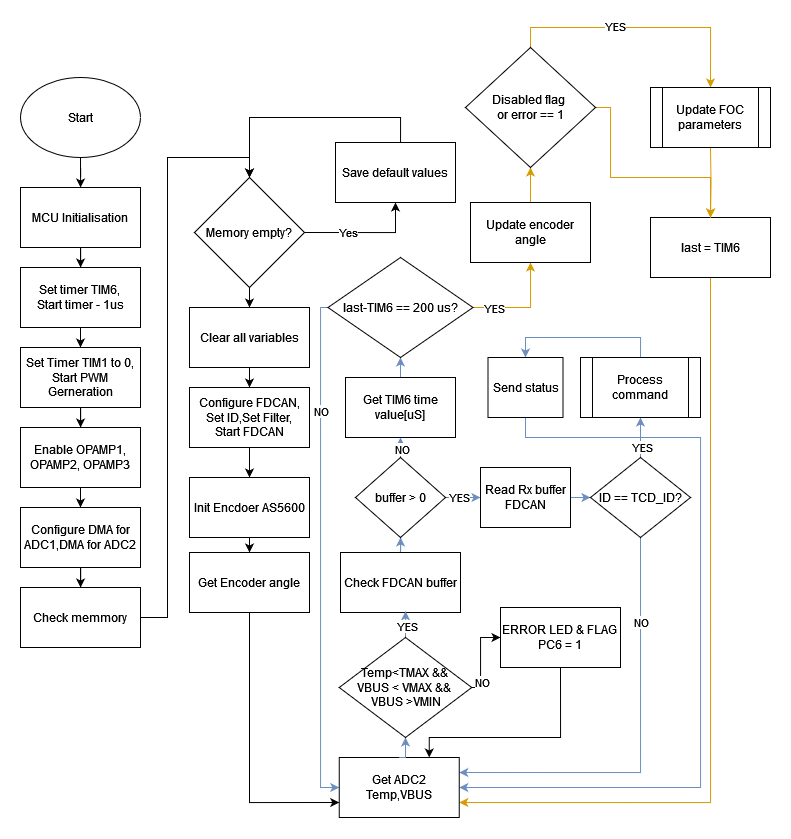
\includegraphics[width=\textwidth]{Src/images/ACD ALG.png}
	\caption{Алгоритм работы системы исполнительной системы.}
	\label{ACDALG}
\end{figure}

После включения микроконтроллер проводит проверку всех устройств на работоспособность путем считывания данных. Система разделена  на две части, в первой части выполняются функци, которые не требуют частого выполнения (окрашено желтым цветом), вторая выполняется на максимальной большой частоте, с которой возможно выполнение, такими задачами являются вычисление векторного алгоритма и парсинг сообщений Рисунок \ref{ACDCMDALG}.

\begin{figure}[H]
	\centering
	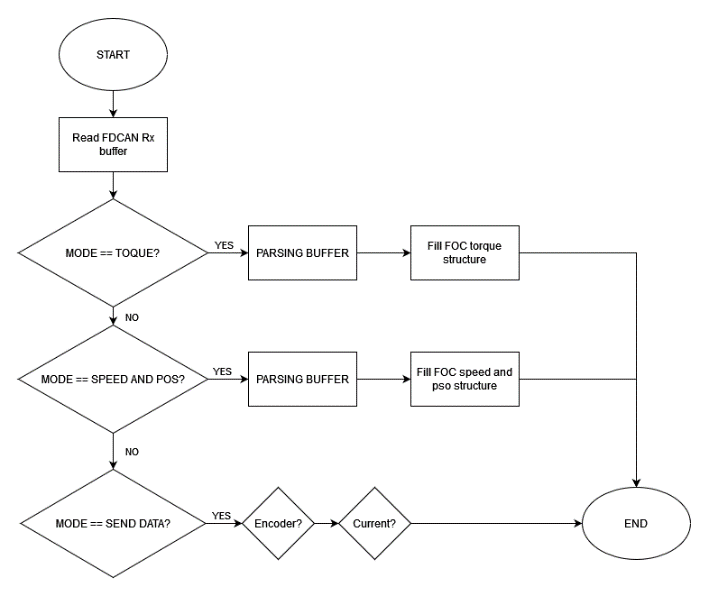
\includegraphics[width=\textwidth]{Src/images/ACDCMDALG.png}
	\caption{Алгоритм обработки сообщения.}
	\label{ACDCMDALG}
\end{figure}

Рисунок 5.8 показывает схема работы векторного регулирования. В качестве примера произведен пример управления по току с обратной связью, что означает, что двигатель всегда создает постоянный крутящий момент (то есть постоянный ток, поскольку крутящий момент пропорционален току).

Входы $i_q$ и $i_d$ регулируются с помощью обратной связи через ПИД-регулятор, который также включает в себя несколько модулей преобразования «Park» и «Clark», сигналы проходят через блок «SVPWM» (Ananth, 2012)(Широтно-импульсная модуляция с пространственным вектором) и происходит воздействие на трехфазный инвертор для управления двигателем, а величина обратной связи ПИД-регулятора представляет собой выборочное значение выходного тока двигателя.

\begin{figure}[H]
	\centering
	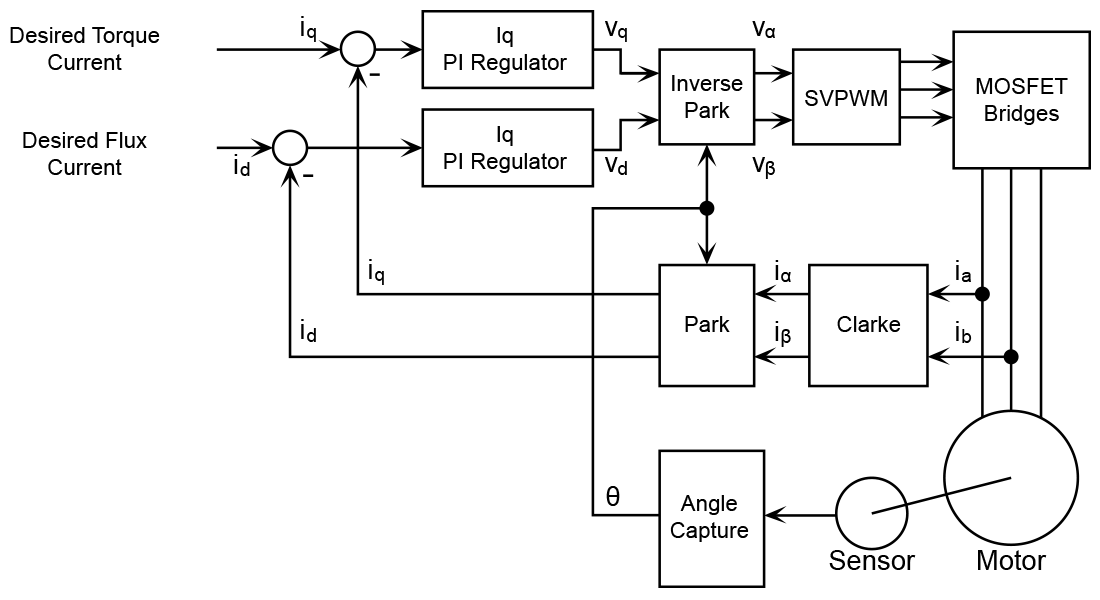
\includegraphics[width=\textwidth]{Src/images/FOCALG.png}
	\caption{Схема векторного управления двигателем.}
	\label{ACDFOCALG}
\end{figure}


Весь процесс векторного управления можно разбить на этапы:
\begin{enumerate}
	\item Получение данных трехфазного тока двигателя для вычисления значений $I_a,I_b$;
	\item Преобразование $I_a,I_b,I_c$ методом Clark, получение $I_\alpha,I_\beta$;
	\item Преобразование $I_\alpha,I_\beta$ методом Park, получение $I_q,I_d$;
	\item Вычисление ошибки $I_q,I_d$; из значений установки $I_q,I_d$ поступающих от контроллера;
	\item Ведение указанной ошибки в два ПИД-регулятора (используется только ПИ), для получения выходных управляющих напряжений $V_q,V_d$;
	\item Преобразование $V_q,V_d$ методом обратным превращением Park, получение $V_\alpha,V_\beta$;
	\item Использование пространственного вектора $V_\alpha,V_\beta$ для определения сигналов широтно-импульсной модуляции для трех полумостов инвертора;
	\item Управление силовыми MOSFET транзисторами трехфазного инвертора в соответствии с ранее выведенным кодовым значением для привода двигателя;
	\item Повторение вышеуказанных шагов;
\end{enumerate}

В вычислениях достаточно использовать только ток с двух фаз мотора, так как по закону тока Кирхгофа можно рассчитать третью составляющую тока, ведь сумма токов, втекающих в узел, равна сумме токов, вытекающих из узла $I_a+I_b+I_c=0$. Вектора $I_a,I_b,I_c$ изначально не ортогональны, для дальнейшей работы требуется провести перерасчет проекции в оси координат, формула \ref{Clark}.
\begin{ceqn}
	\begin{align} \label{Clark}
		\begin{cases}
			I_{\alpha} = I_a - \cos\left(\frac{2\pi}{3}\right) I_b - \cos\left(\frac{2\pi}{3}\right) I_c \\
			I_{\beta} = \sin\left(\frac{2\pi}{3}\right) I_b - \sin\left(\frac{2\pi}{3}\right) I_c
		\end{cases}
	\end{align}
\end{ceqn}

После преобразования получается синусоидальная волна, но на одну переменную меньше. Теперь можно использовать значения $I_\alpha,I_\beta$ для управления вращением двигателя, заставляя их соответствовать правилам изменения формы сигнала. Для применения к трем фазам двигателя применяется обратное преобразование Кларка.
Преобразование Park, формула \ref{Park}, главная задача перевести стационарную систему $I_\alpha,I_\beta$ в cистему координат вращающейся вместе с ротором $I_q,I_d$, а так как в системе подразумевается получать данные положения угла поворота двигателя с энкодера в реальном времени. Получается, что вектор вращения становится фиксированным значением в системе координат$I_\alpha,I_\beta$.  Далее использование $I_q,I_d$ в качестве объектов управления как обратную связь через ПИД-регулятор. В реальности используется только ПИ-регулятор, дифференциальный регулятор не вводится, потому как передаточная функция напряжения и тока является инерционным звено первого порядка.

\begin{ceqn}
	\begin{align} \label{Park}
		\begin{cases}
			I_d = I_\alpha \cos(\theta) + I_\beta \sin(\theta) \\
			I_q = -I_\alpha \sin(\theta) + I_\beta \cos(\theta)
		\end{cases}
	\end{align}
\end{ceqn}


В векторным управлении в основном используются три контура ПИД: контур тока , контур скорости и контур положения, то есть: управление током двигателя (крутящим моментом) посредством обратной связи по току -> затем управление скоростью двигателя, контролируя крутящий момент -> затем управление положением двигателя, контролируя скорость двигателя . 